\documentclass[12pt,a4paper]{article}
\usepackage[utf8]{inputenc}
\usepackage{geometry}
\usepackage{graphicx}
\usepackage{amsmath}
\usepackage{hyperref}
\usepackage{lipsum}
\usepackage{titlesec}
\usepackage{booktabs}
\usepackage{changepage}
\usepackage{caption}
\usepackage{longtable}
\geometry{a4paper, margin=1in}
\setlength{\LTcapwidth}{\textwidth}


% Page layout
\geometry{top=1in, bottom=1in, left=1in, right=1in}

% Title settings
% \title{\textbf{Deep Learning Course \\ Final Project Report}}
% \author{Nama 1 (NIM)\\ Nama 2 (NIM)}
% \date{\today}


% % Modify section and subsection font size to normal
% \titleformat{\section}[hang]{\normalsize\bfseries}{\thesection}{1em}{}
% \titleformat{\subsection}[hang]{\normalsize\bfseries}{\thesubsection}{1em}{}


\begin{document}
% Title
\begin{titlepage}
    \centering
    {\Large\textbf{Deep Learning Course \\ Final Project Report}\par} % Judul
    \vspace{2cm} % Jarak antara judul dan logo
    
    % Menampilkan gambar tanpa lingkungan figure
    
\includegraphics[width=0.5\linewidth]{Image/Logo-Resmi-Unhas.png}\par
    \vspace{2cm} % Jarak antara logo dan nama
    
    {\large
    Ayu Widianti - H071221056\\
    Andi Adnan - H071221078 \\
    Muh. Yusuf Fikry - H071221102\par}
    
    \vspace{1cm} % Jarak antara nama dan tanggal
    {\large\today\par} % Tanggal
\end{titlepage}

\normalsize  % Set the text size to normal for the entire document

% \maketitle
\tableofcontents
\newpage

% 1. Introduction
\section{INTRODUCTION}
\subsection{Background and context}

\begin{adjustwidth}{3em}{0pt} 
\hspace{0.5cm} Pengaduan publik adalah salah satu mekanisme penting dalam mendukung transparansi dan akuntabilitas pemerintah serta organisasi layanan publik. Sistem pengaduan yang efektif memungkinkan masyarakat untuk menyampaikan keluhan, aspirasi, atau masukan terkait berbagai aspek layanan publik. Namun, salah satu tantangan dalam pengelolaan pengaduan adalah mengorganisasi dan mengelompokkan laporan berdasarkan jenis permasalahan yang dilaporkan. Proses ini biasanya memerlukan keterlibatan manual yang memakan waktu dan dapat menghambat respons yang cepat.
 
\hspace{0.5cm} Dalam konteks ini, penggunaan teknologi deep learning menawarkan solusi yang inovatif dan efisien. Dengan memanfaatkan kemampuan model deep learning untuk memahami teks secara mendalam, pengaduan publik dapat diklasifikasikan secara otomatis ke dalam kategori yang relevan, seperti Infrastruktur dan Fasilitas Umum, Kesehatan, atau Pendidikan. Pendekatan ini tidak hanya mempercepat proses pengelompokan laporan tetapi juga mengurangi beban kerja manusia dan meningkatkan pengalaman pengguna dengan meminimalkan input manual.

\hspace{0.5cm} Selain itu, pengembangan model klasifikasi ini memiliki potensi besar untuk diimplementasikan dalam sistem atau aplikasi pengaduan publik. Dengan kemampuan untuk secara otomatis mengkategorikan pengaduan berdasarkan isi laporan, sistem dapat membantu administrator dalam menyusun prioritas penanganan dan membantu pelapor dengan memberikan pengalaman yang lebih sederhana dan efisien. Hal ini sejalan dengan prinsip user-centric design, di mana semakin sedikit input yang diperlukan dari pengguna, semakin mudah dan nyaman penggunaannya.
\end{adjustwidth}

\subsection{Problem statement}
\begin{enumerate}
  \item Kurangnya Dataset Pengaduan Masyarakat yang Terstruktur dan Representatif
  \begin{adjustwidth}{0em}{0pt} 
  Pengaduan masyarakat sering kali tersebar di berbagai platform digital dengan format data yang tidak seragam dan kurang terorganisir. Selain itu, tidak adanya pengelompokan yang komprehensif ke dalam kategori utama seperti pendidikan, infrastruktur, atau kesehatan, membuat analisis data menjadi sulit dilakukan secara efektif.
  \end{adjustwidth}
  \item Kualitas Data yang Tidak Memadai untuk Melatih Model AI
  \begin{adjustwidth}{0em}{0pt} 
  Data pengaduan yang tersedia saat ini sering kali memiliki label kategori yang tidak akurat atau tidak konsisten. Hal ini menghambat pelatihan model kecerdasan buatan, seperti Deep Learning, yang membutuhkan dataset berkualitas tinggi untuk mencapai hasil yang optimal.
  \end{adjustwidth}
  \item Kebutuhan Akan Sistem Otomatis yang Efisien
  \begin{adjustwidth}{0em}{0pt} 
  Dengan meningkatnya volume pengaduan masyarakat, pengelolaan secara manual menjadi tidak efisien dan memakan waktu. Namun, pengembangan sistem otomatis yang mampu menganalisis dan mengklasifikasikan pengaduan dengan cepat terhambat oleh keterbatasan dataset yang relevan dan berkualitas.
  \end{adjustwidth}
\end{enumerate}


\subsection{Objectives of the research}
\begin{enumerate}
  \item Menyusun Dataset yang Terstruktur dan Representatif
  \begin{adjustwidth}{0em}{0pt} 
  Mengembangkan sebuah dataset pengaduan masyarakat yang dirancang secara sistematis dan terorganisir, mencakup 9 kategori utama seperti Infrastruktur dan Fasilitas Umum, Keadilan Hukum dan HAM, Kepegawaian, Kesehatan, Ketenagakerjaan dan Kesejahteraan Sosial, Lingkungan Hidup, Pendidikan, Pertanahan dan Perizinan, serta Teknologi Informasi dan Komunikasi. Dataset ini diharapkan mampu merepresentasikan berbagai bentuk pengaduan masyarakat secara komprehensif, sehingga mencerminkan kebutuhan dan tantangan yang ada di berbagai sektor.\end{adjustwidth}
  
  \item Menghasilkan Dataset Berkualitas Tinggi
  \begin{adjustwidth}{0em}{0pt} 
  Menghasilkan dataset dengan label kategori yang akurat, konsisten, dan bebas dari bias melalui proses anotasi manual yang teliti serta validasi antar annotator. Kualitas dataset ini akan menjadi dasar yang kuat untuk mendukung pelatihan model kecerdasan buatan, seperti Deep Learning, yang membutuhkan data yang relevan dan andal untuk menghasilkan klasifikasi yang tepat dan akurat\end{adjustwidth}
  
  \item Mendukung Pengembangan Sistem Otomatis
  \begin{adjustwidth}{0em}{0pt} 
  Memfasilitasi pengembangan sistem otomatis berbasis kecerdasan buatan yang dapat menganalisis dan mengklasifikasikan pengaduan masyarakat secara efisien. Dataset ini akan menjadi landasan untuk melatih model AI yang mampu menangani volume pengaduan yang besar, memproses data dengan cepat, dan memberikan hasil klasifikasi yang relevan. Dengan demikian, sistem ini diharapkan dapat mempercepat proses pengambilan keputusan dan peningkatan kualitas pelayanan publik.
  \end{adjustwidth}
\end{enumerate}




% \noindent Example:
% \lipsum[1] % Replace this with your content.

% 2. Related Works
\section{Related Works}
\subsection{Literature review of relevant papers and articles}
\begin{adjustwidth}{3em}{0pt} 
\hspace{0.5cm} Dalam literatur pertama yang mengaplikasikan \textit{Long Short-Term Memory} (LSTM) untuk klasifikasi laporan masyarakat di platform LAPOR!, penulis menyoroti efisiensi LSTM dalam mengelola data teks berurutan. Metode ini menggunakan teknik scraping untuk mengumpulkan laporan yang telah diverifikasi, kemudian diproses dengan REST API untuk klasifikasi. Hasil yang diperoleh menunjukkan bahwa LSTM cukup efektif dalam menangani tugas klasifikasi pengaduan masyarakat. Namun, penulis menyarankan evaluasi lebih lanjut terhadap model lain guna mengoptimalkan hasil klasifikasi, serta untuk menangani kemungkinan tantangan yang dihadapi dalam pemrosesan teks berurutan yang lebih kompleks(Rozi et al.2020)

\hspace{0.5cm} Penelitian pada literatur ke-2 menguji metode Multinomial Naïve Bayes yang dipadukan dengan teknik N-gram untuk klasifikasi pengaduan di platform SAMBAT Online. Dalam eksperimen ini, penggunaan unigram menghasilkan akurasi tinggi sebesar 88,23\%, dengan akurasi rata-rata mencapai 80,88\%. Penulis menunjukkan bahwa meskipun metode ini cukup efektif, hasil klasifikasi sangat bergantung pada kualitas dan variabilitas dataset yang digunakan. Penelitian ini juga mencatat bahwa meskipun penambahan N-gram memberikan sedikit peningkatan, seleksi fitur yang lebih cermat dan pengembangan lebih lanjut terhadap metode klasifikasi lain perlu dilakukan untuk memperbaiki hasil yang diperoleh.(Saputra et al.2020)

\hspace{0.5cm} Pada penelitian ketiga, penggunaan Neural Network untuk klasifikasi pengaduan masyarakat menghasilkan hasil yang kurang memuaskan, dengan akurasi hanya mencapai 43\%. Selain itu, waktu pemrosesan yang dibutuhkan cukup lama, yaitu 3 jam 45 menit 14 detik. Penelitian ini menunjukkan bahwa meskipun Neural Network memiliki potensi, performanya masih rendah dan memerlukan pengoptimalan lebih lanjut. Penulis merekomendasikan pengujian dengan algoritma lain yang mungkin lebih efisien dan dapat memberikan akurasi lebih tinggi serta proses klasifikasi yang lebih cepat.(yuliana et al.2019)

\hspace{0.5cm} Tinjauan literatur dari ketiga penelitian ini mengungkapkan bahwa setiap pendekatan memiliki kelebihan dan kekurangannya masing-masing. LSTM efektif dalam menangani teks berurutan, namun pengujian lebih lanjut perlu dilakukan untuk meningkatkan kinerjanya. Metode Naïve Bayes dengan N-gram menawarkan akurasi yang baik, namun sangat dipengaruhi oleh kualitas data dan pemilihan fitur. Di sisi lain, Neural Network, meskipun populer dalam tugas klasifikasi teks, menunjukkan performa yang kurang optimal dalam konteks pengaduan masyarakat, yang menunjukkan bahwa algoritma lain mungkin lebih cocok untuk tugas ini. Penelitian-penelitian ini memberikan wawasan penting dalam pemilihan dan pengembangan metode klasifikasi yang lebih efektif dalam konteks pengaduan masyarakat berbasis platform digital.
\end{adjustwidth}

\subsection{Comparison of different approaches and their results}

\begin{adjustwidth}{3em}{0pt} 
\hspace{0.5cm} Perbandingan metode yang digunakan dalam ketiga penelitian menunjukkan kelebihan dan kekurangan masing-masing. LSTM terbukti efektif dalam menangani teks berurutan dan memberikan hasil yang baik untuk klasifikasi laporan masyarakat, tetapi masih memerlukan pengujian lebih lanjut untuk mengoptimalkan performa. Multinomial Naïve Bayes dengan N-gram memberikan hasil terbaik dengan akurasi 88,23\%, meskipun ketergantungan pada kualitas data cukup tinggi. Meskipun kombinasi N-gram membantu, seleksi fitur yang lebih baik diperlukan untuk hasil yang lebih optimal. Di sisi lain, penggunaan Neural Network menghasilkan akurasi yang rendah (43,00\%) dan waktu yang lebih lama, yang menandakan bahwa algoritma ini perlu dioptimalkan atau diganti dengan metode yang lebih efisien dan efektif untuk tugas klasifikasi teks pengaduan masyarakat.
\end{adjustwidth}

\subsection{Justification for your chosen methodology}
\begin{adjustwidth}{3em}{0pt} 
\hspace{0.5cm} Dalam pengembangan dataset ini, Pemilihan LSTM (Long Short-Term Memory), IndoBERT, dan XLM-RoBERTa sebagai metodologi dalam penelitian ini didasarkan pada kelebihan masing-masing model yang sesuai dengan karakteristik data teks pengaduan masyarakat dalam Bahasa Indonesia.
\begin{itemize}
    \item LSTM (\textit{Long Short-Term Memory}) adalah jenis \textit{Recurrent Neural Network} (RNN) yang dirancang untuk mempelajari dependensi jangka panjang dalam data sekuensial. Metode ini efektif untuk mengklasifikasikan teks berurutan, di mana urutan kata penting untuk memahami makna. Dalam konteks pengaduan masyarakat, LSTM dapat menangani teks yang panjang dan kompleks, seperti laporan pengaduan yang memiliki pola komunikasi tertentu yang perlu ditangkap untuk klasifikasi yang akurat.
    \item \textit{IndoBERT} adalah model berbasis Transformer, yang merupakan arsitektur state-of-the-art dalam pemrosesan bahasa alami (Natural Language Processing). Arsitektur Transformer diperkenalkan melalui penelitian Vaswani et al. (2017) dan telah merevolusi cara model menangkap hubungan dalam data sekuensial. Salah satu komponen utama dalam arsitektur ini adalah mekanisme self-attention, yang memungkinkan model untuk secara efektif mempelajari hubungan antara kata-kata dalam suatu kalimat, terlepas dari jarak antar kata tersebut.Dengan menggunakan IndoBERT, model dapat lebih baik menangkap konteks semantik dalam teks Bahasa Indonesia, yang sangat penting untuk mengklasifikasikan laporan pengaduan masyarakat yang beragam. IndoBERT juga lebih efisien dalam menangani ekspresi khas dalam bahasa lokal yang mungkin tidak dapat dipahami oleh model berbasis bahasa lain. 
    \item \textit{XLM-RoBERTa}, yang merupakan model multibahasa, memiliki keunggulan dalam memahami teks dalam berbagai bahasa, termasuk Bahasa Indonesia. Ini sangat berguna apabila terdapat campuran bahasa atau teks yang menggunakan elemen dari bahasa lain selain Bahasa Indonesia. XLM-RoBERTa mampu memanfaatkan berbagai sumber data bahasa untuk meningkatkan kemampuan klasifikasi, menjadikannya pilihan yang baik untuk menangani variasi dalam dataset pengaduan masyarakat yang berpotensi mengandung elemen-elemen bahasa campuran.
\end{itemize}
\end{adjustwidth}

% 3. Dataset and Material
\section{Dataset and Material}

\subsection{Source of the Dataset}
\begin{adjustwidth}{3em}{0pt} 
\hspace{0.5cm} Dalam pengembangan dataset\textit{ "Public Complain",} data diambil dari platform pengaduan publik resmi \textit{lapor.go.id}, sebuah sistem nasional yang dirancang untuk mengelola dan menampung keluhan masyarakat. Situs ini menjadi sumber data utama karena menyediakan berbagai pengaduan yang mencakup kategori relevan dengan kebutuhan projek ini, seperti pendidikan, infrastruktur, kesehatan, ekonomi, sosial, dan pelayanan publik lainnya. Laporan yang diunggah oleh masyarakat ke dalam situs ini mencerminkan permasalahan nyata yang dihadapi di berbagai sektor, sehingga memberikan representasi data yang mendalam dan kaya untuk keperluan pengembangan dataset.

\hspace{0.5cm} 
Pengumpulan data dilakukan dengan menggunakan teknik \textit{web scraping}, yaitu proses otomatisasi pengambilan data dari situs web. Teknik ini dipilih karena mampu menangani volume data yang besar secara efisien dan memungkinkan pengelompokan data berdasarkan kategori yang spesifik. Setiap pengaduan yang diambil diproses dan dikelompokkan berdasarkan kategori utama yang telah ditentukan. Data yang dikumpulkan meliputi detail laporan yaitu judul pengaduan dan isi laporan, serta kategori tertentu. Hal ini memastikan dataset yang dihasilkan memiliki struktur yang jelas dan dapat digunakan untuk berbagai kebutuhan analisis.\end{adjustwidth}

\begin{figure} % Menggunakan [H] agar gambar tetap di tempat
    \centering
    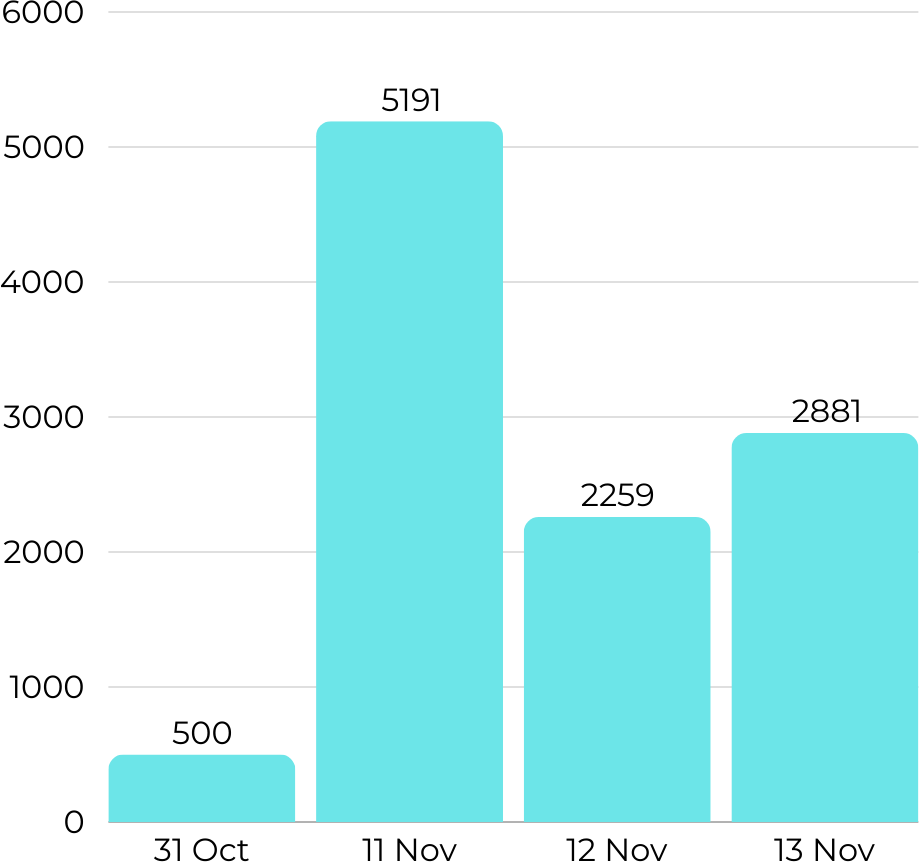
\includegraphics[width=0.5\linewidth]{Image/progress pengumpulan data.png}
    \caption{Gambar 3.1 Progress Pengumpulan Data}
    \label{fig:roc_auc}
\end{figure}  

\begin{figure} % Menggunakan [H] agar gambar tetap di tempat
    \centering
    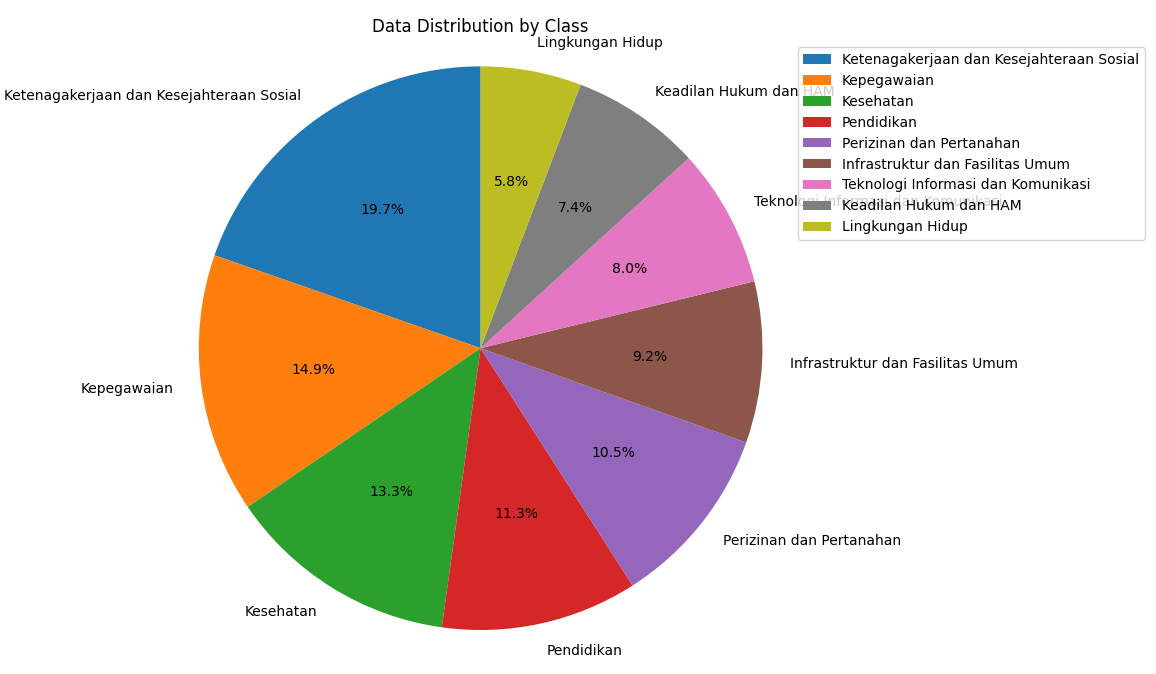
\includegraphics[width=0.5\linewidth]{Image/data distribution by class.png}
    \caption{Gambar 3.2 Data Distribution by Class}
    \label{fig:roc_auc}
\end{figure} 

\begin{itemize}
    \begin{itemize}
        \item Total data : 10.831
        \item Pekan 11 : 500 data
        \item Pekan 12 : 0 data
        \item Pekan 13 : 10.331 data
    \end{itemize}
\end{itemize}

\newpage
\subsection{Preprocessing Steps}
\begin{adjustwidth}{3em}{0pt} \hspace{0.5cm} Tahapan data preprocessing merupakan tahapan pembersihan data untuk meminimalisir atau menghilangkan \textit{noise}. Proses data \textit{preprocessing} sangat penting untuk mendapatkan akurasi model terbaik (Lubis et al., 2023). Langkah-langkah yang dilakukan untuk mempersiapkan data teks agar siap digunakan dalam pelatihan model deteksi komentar negatif. Proses ini bertujuan untuk membersihkan, menormalisasi, dan menyederhanakan data teks agar lebih mudah dianalisis dan dipahami oleh model. \end{adjustwidth}

\subsubsection{Lower Casing}
\begin{adjustwidth}{3em}{0pt} \hspace{0.5cm} Langkah pertama dalam preprocessing adalah \textit{lower casing}, yaitu mengubah semua teks dalam dataset menjadi huruf kecil (lowercase). Hal ini dilakukan untuk mengatasi perbedaan dalam pengenalan kata akibat penggunaan kapitalisasi yang tidak konsisten, misalnya kata "Pendidikan" dan "pendidikan" akan dianggap berbeda jika tidak diubah. Dengan melakukan lower casing, kita memastikan bahwa variasi kapitalisasi tidak mempengaruhi analisis teks dan model dapat mengenali kata yang sama tanpa terpengaruh perbedaan format. \end{adjustwidth}

\subsubsection{Cleaning Text}
\begin{adjustwidth}{3em}{0pt} \hspace{0.5cm} \textit{Cleaning text} merupakan langkah pembersihan data yang bertujuan untuk menghilangkan elemen-elemen yang tidak relevan atau mengganggu dalam teks, sehingga dapat meningkatkan kualitas analisis.Pada dataset pengaduan masyarakat, teks sering kali mengandung elemen ini, misalnya "Fasilitas rusak di jalan tol!!! \textit{www.contohurl.com}". Proses ini mencakup penghapusan tanda baca seperti titik, koma, tanda tanya, dan sebagainya, yang tidak memberikan makna dalam konteks analisis teks. Selain itu, URL atau tautan yang terdapat dalam teks juga dihapus karena tidak berkontribusi terhadap makna atau analisis. Angka dan karakter spesial yang tidak diperlukan dalam konteks pemrosesan teks juga dihilangkan, sehingga teks menjadi lebih bersih dan fokus pada informasi yang relevan untuk model klasifikasi. \end{adjustwidth}

\subsubsection{Normalization}
\begin{adjustwidth}{3em}{0pt} \hspace{0.5cm} \textit{Normalization} adalah proses untuk mengubah teks yang tidak baku atau tidak konsisten menjadi bentuk yang lebih standar atau baku. Normalisasi digunakan untuk menyamakan variasi ejaan atau penggunaan kata dengan makna yang sama, seperti "tdk" menjadi "tidak" atau "gak" menjadi "tidak". Dalam pengaduan masyarakat, variasi bahasa informal sering ditemukan, terutama di kategori seperti Lingkungan Hidup atau Kesehatan. \end{adjustwidth}

\subsubsection{Remove Stopwords}
\begin{adjustwidth}{3em}{0pt} \hspace{0.5cm} Pada Tahap ini adalah menghapus kata-kata umum seperti "yang", "dan", atau "adalah", yang tidak memberikan informasi signifikan dalam pengolahan teks. Pada dataset pengaduan masyarakat, stopwords sering kali mendominasi teks keluhan, misalnya dalam kalimat "Jalan yang rusak di daerah saya sudah lama tidak diperbaiki". Dengan menghapus stopwords, fokus analisis dapat dialihkan ke kata-kata yang memiliki bobot lebih penting, seperti "jalan", "rusak", dan "daerah".\end{adjustwidth}

\subsection{Features and labels}
\begin{adjustwidth}{3em}{0pt} 
\hspace{0.5cm} Fitur dalam dataset ini adalah atribut atau informasi yang menjadi masukan bagi model untuk memahami dan memproses data pengaduan masyarakat secara otomatis. Fitur-fitur ini dirancang untuk memberikan konteks dan informasi yang relevan, sehingga membantu model dalam melakukan analisis dan klasifikasi pengaduan.
\begin{itemize}
    \item Link : berisi tautan sumber pengaduan, yang menunjukkan dari mana data diambil. Link berfungsi sebagai pengenal unik untuk setiap entri pengaduan, sehingga memungkinkan pengguna atau peneliti melacak kembali informasi asli ke sumbernya. 
    \item Judul Pengaduan : Teks pengaduan adalah elemen utama dalam dataset yang berisi deskripsi keluhan masyarakat. 
    \item Konten : Atribut ini mencakup isi lengkap dari pengaduan masyarakat, yang berisi detail rinci mengenai masalah yang dihadapi.
\end{itemize}

\hspace{0.5cm} Dalam pengembangan dataset ini target atau output kategori pengaduan yang menjadi hasil akhir yang ingin diprediksi atau diklasifikasikan, yaitu :

\begin{itemize}
    \item \textit{Infrastruktur dan Fasilitas Umum}: Masalah jalan, transportasi, atau fasilitas publik.
    \item \textit{Keadilan Hukum dan HAM}: Keluhan tentang pelanggaran hukum atau HAM.
    \item \textit{Kepegawaian}: Masalah terkait pegawai pemerintah atau swasta.
    \item \textit{Kesehatan}: Keluhan tentang layanan kesehatan atau fasilitas medis.
    \item \textit{Kesehatan}: Keluhan tentang layanan kesehatan atau fasilitas medis.
    \item \textit{Ketenagakerjaan dan Kesejahteraan Sosial}: Masalah terkait pekerjaan atau jaminan sosial.
    \item \textit{Lingkungan Hidup}: Keluhan tentang kerusakan lingkungan atau polusi.
    \item \textit{Pendidikan}: Masalah dalam sistem atau fasilitas pendidikan.
    \item \textit{Pertanahan dan Perizinan}: Keluhan tentang konflik tanah atau izin usaha.
    \item \textit{Teknologi Informasi dan Komunikasi}: Masalah dengan akses atau infrastruktur teknologi.
\end{itemize}

\end{adjustwidth}
\newpage











% 4. Result and Discussion
\section{Result and Discussion}
\begin{adjustwidth}{3em}{0pt}
\hspace{0.5cm} Berikut adalah hasil evaluasi model pada berbagai kategori berdasarkan metrik Precision, Recall, dan F1-Score. Tabel berikut menunjukkan performa model \textit{LSTM}, \textit{IndoBERT}, dan \textit{XLM-RoBERTa} pada masing-masing kategori, serta perbandingannya terhadap data uji yang tersedia. Perbandingan ini memberikan gambaran mengenai efisiensi dan kecocokan masing-masing model untuk menangani berbagai kategori data.\end{adjustwidth}

\begin{table}[h!]
\centering
\scriptsize % Ukuran lebih kecil untuk tabel
\begin{tabular}{|l|c|c|c|c|c|}
\hline
\textbf{Kategori} & \textbf{Test Data} & \textbf{Metric} & \textbf{LSTM} & \textbf{IndoBERT} & \textbf{XLM-RoBERTa} \\ \hline
Infrastruktur dan Fasilitas Umum & 187 & Precision & 0.80 & 0.90 & 0.84 \\ 
 &  & Recall & 0.88 & 0.95 & 0.93 \\ 
 &  & F1-Score & 0.84 & 0.95 & 0.93 \\ \hline
Keadilan Hukum dan HAM & 163 & Precision & 0.58 & 0.90 & 0.86 \\ 
 &  & Recall & 0.47 & 0.69 & 0.72 \\ 
 &  & F1-Score & 0.52 & 0.78 & 0.79 \\ \hline
Kepegawaian & 316 & Precision & 0.78 & 0.82 & 0.80 \\ 
 &  & Recall & 0.88 & 0.88 & 0.85 \\ 
 &  & F1-Score & 0.83 & 0.85 & 0.82 \\ \hline
Kesehatan & 263 & Precision & 0.79 & 0.87 & 0.89 \\ 
 &  & Recall & 0.76 & 0.87 & 0.83 \\ 
 &  & F1-Score & 0.77 & 0.87 & 0.86 \\ \hline
Ketenagakerjaan dan Kesejahteraan Sosial & 440 & Precision & 0.87 & 0.88 & 0.89 \\ 
 &  & Recall & 0.82 & 0.90 & 0.89 \\ 
 &  & F1-Score & 0.85 & 0.89 & 0.89 \\ \hline
Lingkungan Hidup & 115 & Precision & 0.64 & 0.76 & 0.76 \\ 
 &  & Recall & 0.54 & 0.80 & 0.76 \\ 
 &  & F1-Score & 0.58 & 0.78 & 0.76 \\ \hline
Pendidikan & 243 & Precision & 0.80 & 0.92 & 0.85 \\ 
 &  & Recall & 0.84 & 0.86 & 0.84 \\ 
 &  & F1-Score & 0.82 & 0.89 & 0.85 \\ \hline
Perizinan dan Pertanahan & 226 & Precision & 0.83 & 0.91 & 0.87 \\ 
 &  & Recall & 0.81 & 0.91 & 0.88 \\ 
 &  & F1-Score & 0.82 & 0.91 & 0.87 \\ \hline
Teknologi Informasi dan Komunikasi & 172 & Precision & 0.78 & 0.92 & 0.91 \\ 
 &  & Recall & 0.84 & 0.94 & 0.95 \\ 
 &  & F1-Score & 0.81 & 0.93 & 0.93 \\ \hline
Overall (Weighted Avg) & 2127 & Precision & 0.79 & 0.88 & 0.86 \\ 
 &  & Recall & 0.79 & 0.88 & 0.86 \\ 
 &  & F1-Score & 0.79 & 0.88 & 0.86 \\ \hline
Overall Accuracy &  &  & 0.79 & 0.88 & 0.86 \\ \hline
\end{tabular}
\caption{Tabel Metrics}
\end{table}

\begin{adjustwidth}{3em}{0pt} 
\hspace{0.5cm} Hasil evaluasi dari tiga model deep learning, yaitu LSTM, IndoBERT, dan \textit{XLM-RoBERTa}, menunjukkan bahwa IndoBERT memberikan performa terbaik dalam mengklasifikasikan pengaduan publik berdasarkan kategori yang ada. Berdas-arkan hasil yang tercantum dalam Tabel 1, IndoBERT menghasilkan nilai \textit{precision}, \textit{recall}, dan \textit{F1-Score }tertinggi di sebagian besar kategori, termasuk "Infrastruktur dan Fasilitas Umum" dengan precision 0.90, recall 0.95, dan F1-Score 0.92. Keunggulan \textit{IndoBERT} terlihat pada kemampuannya untuk menangani variasi teks dan konteks yang lebih kompleks, yang berkontribusi pada kemampuan model untuk mengidentifikasi kategori pengaduan dengan akurat dan efisien.

\hspace{0.5cm} \textit{XLM-RoBERTa} juga menunjukkan performa yang sangat baik, terutama pada kategori dengan jumlah data yang lebih besar, seperti "Teknologi Informasi dan Komunikasi" dan "Ketenagakerjaan dan Kesejahteraan Sosial", di mana model ini menghasilkan F1-Score 0.93 dan 0.89. Meskipun \textit{XLM-RoBERTa }unggul dalam kategori-kategori tersebut, secara keseluruhan, IndoBERT tetap lebih unggul karena kestabilannya di hampir semua kategori. Hasil ini menunjukkan bahwa \textit{IndoBERT} tidak hanya mampu mengklasifikasikan dengan akurat, tetapi juga memberikan keseimbangan yang lebih baik antara \textit{precision} dan \textit{recall}, yang sangat penting untuk aplikasi pengaduan publik yang membutuhkan kecepatan dan akurasi dalam penanganan laporan.

\hspace{0.5cm} Sementara itu, \textit{LSTM} menunjukkan hasil yang lebih rendah dibandingkan dengan kedua model berbasis Transformer, baik dalam precision, \textit{recall}, maupun \textit{F1-Score}. LSTM masih memberikan hasil yang cukup baik pada beberapa kategori, tetapi secara keseluruhan, performanya lebih terbatas dibandingkan IndoBERT dan XLM-RoBERTa.\end{adjustwidth}

\begin{adjustwidth}{3em}{0pt} 
    \hspace{0.5cm} Berikut adalah confusion matrix dari tiga model, yaitu IndoBERT, LSTM, dan XLM-RoBERTa, yang menunjukkan performa masing-masing dalam mengklasifikasikan data berdasarkan kategori.
\end{adjustwidth}

\begin{adjustwidth}
    \begin{figure}
    \centering
    \begin{minipage}{0.3\textwidth}
        \centering
        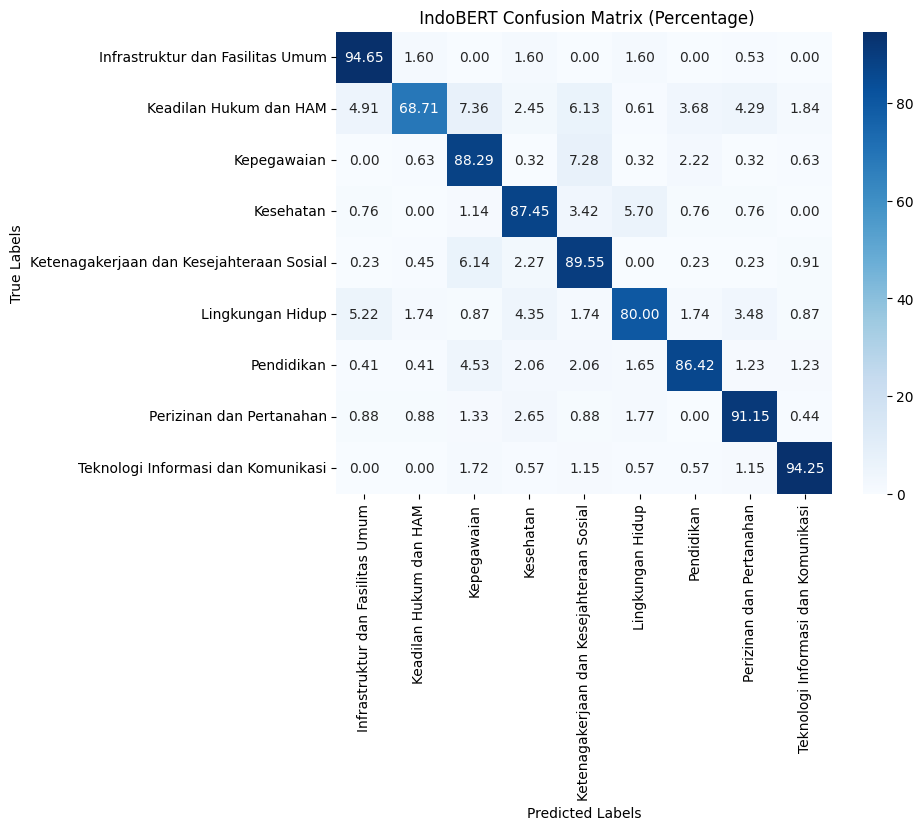
\includegraphics[width=\linewidth]{Image/cm_indobert.png}
        \label{fig:indobert}
    \end{minipage} \hfill
    \begin{minipage}{0.3\textwidth}
        \centering
        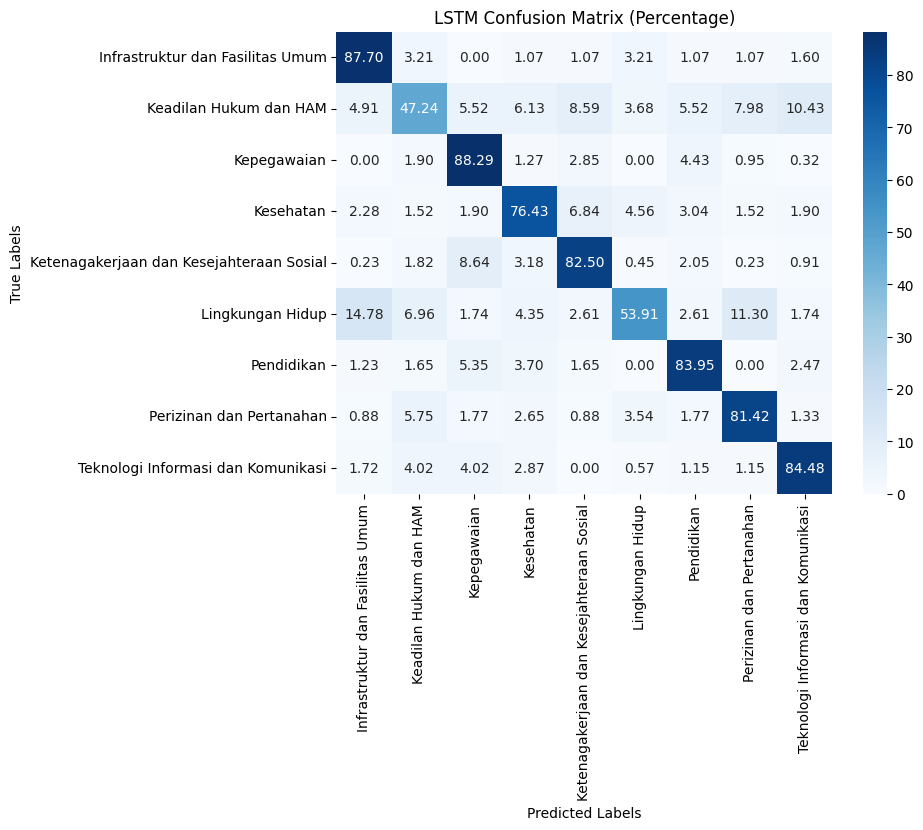
\includegraphics[width=\linewidth]{Image/cm_lstm.png}
        \label{fig:lstm}
    \end{minipage} \hfill
    \begin{minipage}{0.3\textwidth}
        \centering
        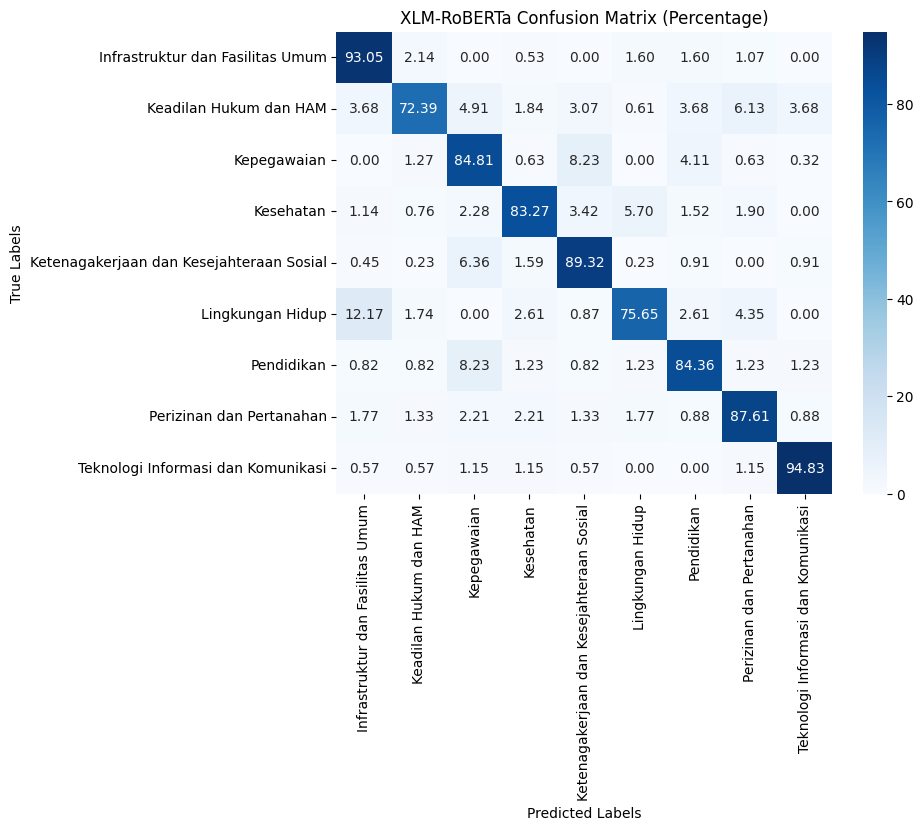
\includegraphics[width=\linewidth]{Image/cm_xlm.png}
        \label{fig:xlm}
    \end{minipage}
    \end{figure}
\end{adjustwidth}
\begin{adjustwidth}{3em}{0pt} 
\hspace{0.5cm} Model IndoBERT menunjukkan performa terbaik di antara ketiga model. Model ini mampu mengklasifikasikan data dengan akurasi tinggi pada hampir semua kategori, seperti Infrastruktur dan Fasilitas Umum (94.65\%), Teknologi Informasi dan Komunikasi (94.25\%), dan Perizinan dan Pertanahan (91.15\%). Namun, kategori seperti Keadilan Hukum dan HAM (68.71\%) memiliki tingkat akurasi lebih rendah dan cenderung sering salah diklasifikasikan ke kategori lain, seperti Kepegawaian dan Lingkungan Hidup. Meski begitu, model ini secara keseluruhan cukup stabil dan efisien dalam mengelola data dengan kompleksitas yang tinggi.

\hspace{0.5cm} Sementara itu, model LSTM menunjukkan performa yang paling rendah di antara ketiga model. Akurasi pada kategori Keadilan Hukum dan HAM (47.24\%) dan Lingkungan Hidup (53.91\%) sangat rendah, dengan banyak kesalahan klasifikasi ke kategori lain, seperti Infrastruktur dan Fasilitas Umum (14.78\%). Meski demikian, LSTM tetap menunjukkan performa yang baik pada kategori Kepegawaian (88.29\%) dan Pendidikan (83.95\%), tetapi secara keseluruhan, model ini tidak dapat menangani data yang lebih kompleks sebaik IndoBERT atau XLM-RoBERTa.

\hspace{0.5cm} Model XLM-RoBERTa memiliki kinerja yang cukup baik, mendekati IndoBERT, dan menunjukkan akurasi tinggi pada kategori seperti Teknologi Informasi dan Komunikasi (94.83\%), Infrastruktur dan Fasilitas Umum (93.05\%), dan Ketenagakerjaan dan Kesejahteraan Sosial (89.32\%). Model ini juga lebih baik dari LSTM dalam menangani kategori yang lebih sulit, seperti Keadilan Hukum dan HAM (72.39\%) dan Lingkungan Hidup (75.65\%), meskipun masih memiliki tingkat kesalahan yang lebih tinggi dibandingkan IndoBERT. Model ini menunjukkan stabilitas yang lebih baik dibandingkan LSTM, tetapi masih memerlukan peningkatan pada beberapa kategori tertentu.

\end{adjustwidth}



\begin{adjustwidth}
\begin{figure}[H]
    \centering
    \begin{minipage}{0.3\textwidth}
        \centering
        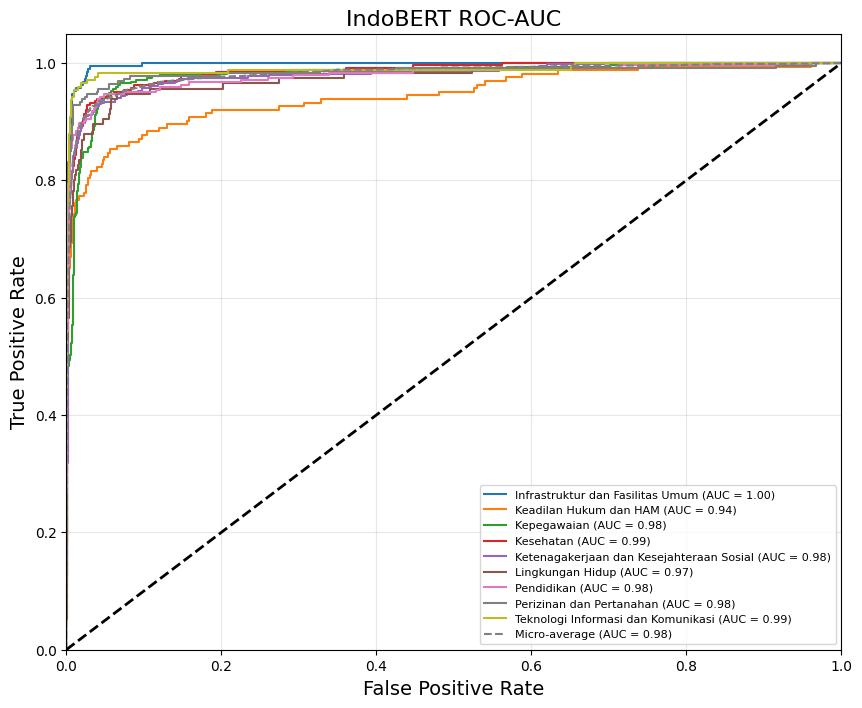
\includegraphics[width=\linewidth]{Image/roc-auc_indobert.png}
        \caption*{Indobert}
        \label{fig:indobert}
    \end{minipage} \hfill
    \begin{minipage}{0.3\textwidth}
        \centering
        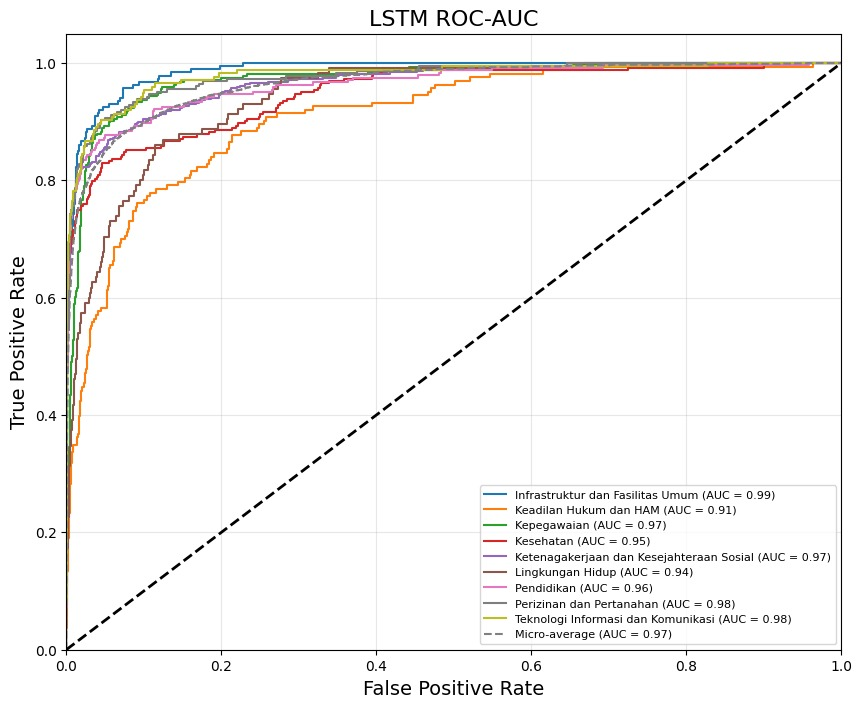
\includegraphics[width=\linewidth]{Image/roc-lstm.jpg}
        \caption*{LSTM}
        \label{fig:lstm}
    \end{minipage} \hfill
    \begin{minipage}{0.3\textwidth}
        \centering
        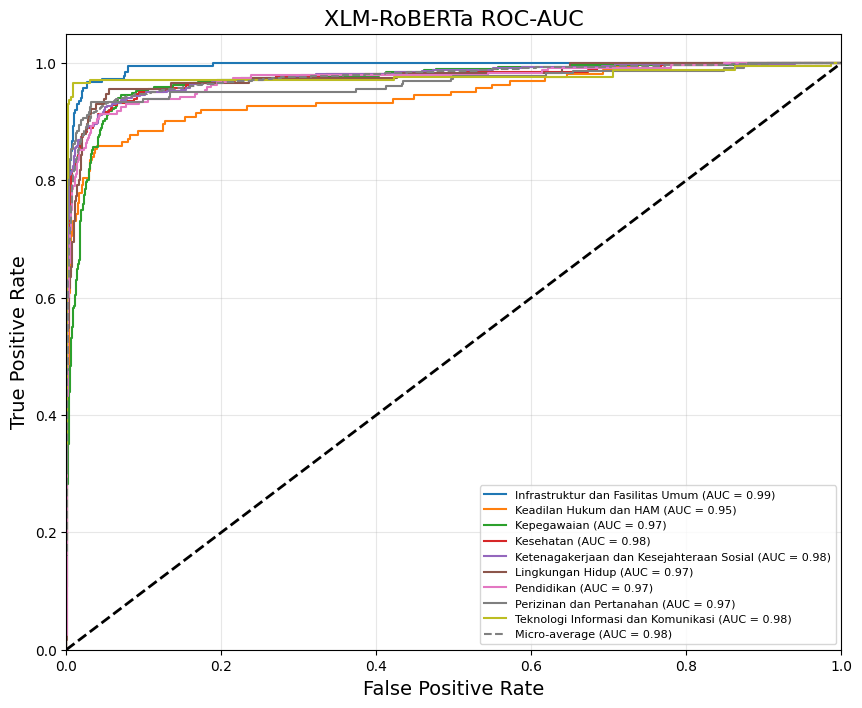
\includegraphics[width=\linewidth]{Image/roc-auc_xlm.png}
        \caption*{XLM}
        \label{fig:xlm}
    \end{minipage}
    \end{figure}
\end{adjustwidth}

\begin{adjustwidth}{3em}{0pt} 
    \hspace{0.5cm} Gambar diatas menunjukkan perbandingan performa tiga model klasifikasi (LSTM, IndoBERT, dan XLM-RoBERTa) berdasarkan kurva ROC-AUC untuk berbagai kategori data. Model IndoBERT menunjukkan performa terbaik dengan nilai AUC hampir sempurna pada sebagian besar kategori, terutama kategori "Infrastruktur dan Fasilitas Umum" (AUC = 1.00), diikuti oleh XLM-RoBERTa dengan performa stabil namun sedikit lebih rendah dibandingkan IndoBERT. Sementara itu, model LSTM memiliki performa yang lebih bervariasi, dengan AUC lebih rendah pada beberapa kategori seperti "Pendidikan dan Penelitian." Secara keseluruhan, IndoBERT unggul dalam membedakan antara kelas, membuatnya menjadi model yang paling andal untuk tugas klasifikasi dalam dataset ini, terutama untuk data pengaduan masyarakat yang beragam.
\end{adjustwidth}

\subsection{Discussion of the result}
\begin{adjustwidth}{3em}{0pt} 
    \hspace{0.5cm} Hasil evaluasi dari tiga model deep learning (LSTM, IndoBERT, dan XLM-RoBERTa) menunjukkan bahwa IndoBERT memberikan performa terbaik dalam mengklasifikasikan pengaduan masyarakat berdasarkan kategori. Keunggulan model ini terlihat pada nilai precision, recall, dan F1-Score yang tinggi di sebagian besar kategori, seperti "Infrastruktur dan Fasilitas Umum" dengan precision 0.90, recall 0.95, dan F1-Score 0.92. Hal ini menunjukkan kemampuan IndoBERT dalam menangani variasi teks dan konteks yang kompleks, yang sejalan dengan kebutuhan aplikasi pengaduan masyarakat yang memprioritaskan akurasi dan efisiensi dalam pengolahan data.

    \hspace{0.5cm} Dibandingkan dengan penelitian oleh Rozi et al. (2020) yang menggunakan LSTM, hasil pada penelitian ini menunjukkan bahwa meskipun LSTM cukup efektif dalam menangani teks berurutan, performanya masih kalah dari model berbasis transformer seperti IndoBERT dan XLM-RoBERTa. Pada penelitian Rozi, LSTM direkomendasikan untuk dievaluasi lebih lanjut dengan model lain, yang terbukti relevan mengingat IndoBERT memberikan hasil yang jauh lebih unggul pada dataset dengan kompleksitas yang lebih tinggi.

    \hspace{0.5cm} Hasil XLM-RoBERTa pada penelitian ini juga menarik karena model ini menunjukkan performa yang sangat baik pada kategori dengan jumlah data lebih besar, seperti "Teknologi Informasi dan Komunikasi" dan "Ketenagakerjaan dan Kesejahteraan Sosial." Temuan ini sejalan dengan kemampuan Naïve Bayes berbasis N-gram yang diuji dalam penelitian Saputra et al. (2020), di mana akurasi tertinggi dicapai pada dataset yang terstruktur dengan baik. Namun, dibandingkan dengan XLM-RoBERTa, model transformer ini menunjukkan stabilitas yang lebih baik pada hampir semua kategori, menandakan keunggulannya dalam menangani data dengan variasi konteks lebih luas.

    \hspace{0.5cm} Sementara itu, LSTM pada penelitian ini menunjukkan performa yang lebih rendah, dengan tingkat kesalahan klasifikasi yang cukup tinggi pada kategori seperti "Keadilan Hukum dan HAM" dan "Lingkungan Hidup." Hal ini konsisten dengan temuan dari Yuliana et al. (2019), di mana Neural Network tradisional menunjukkan akurasi yang rendah (43\%) dalam tugas klasifikasi pengaduan masyarakat. Keterbatasan ini menunjukkan bahwa arsitektur berbasis RNN, termasuk LSTM, memiliki kelemahan dalam menangani data dengan kompleksitas tinggi dibandingkan dengan model transformer modern.

    \hspace{0.5cm} Dari hasil dan tinjauan literatur, terlihat bahwa IndoBERT berhasil mengatasi keterbatasan pendekatan terdahulu, terutama dalam hal akurasi, stabilitas, dan efisiensi waktu pemrosesan. Dengan AUC yang hampir sempurna dan performa yang konsisten di hampir semua kategori, IndoBERT tidak hanya memenuhi kebutuhan klasifikasi pengaduan masyarakat tetapi juga memberikan standar baru untuk pengembangan model berbasis Bahasa Indonesia. Model XLM-RoBERTa, meskipun memiliki performa mendekati IndoBERT, masih memerlukan optimalisasi pada beberapa kategori untuk mencapai tingkat akurasi yang lebih konsisten. Adapun LSTM, meskipun tetap relevan untuk tugas-tugas tertentu, terbukti kurang kompetitif dalam konteks ini dibandingkan kedua model transformer
\end{adjustwidth}













% \noindent Example:
% \begin{itemize}
%     \item \textbf{Accuracy:} 95.2\%
%     \item \textbf{Precision:} 94.8\%
%     \item \textbf{Recall:} 96.0\%
% \end{itemize}

% \begin{figure}[h!]
%     \centering
%     \includegraphics[width=0.8\textwidth]{example-result.png} % Replace with your image
%     \caption{Example Result Visualization}
%     \label{fig:result}
% \end{figure}

% 5. Conclusion
\newpage
\section{Conclusion}
\begin{adjustwidth}{3em}{0pt} 
    \hspace{0.5cm} Proyek ini bertujuan mengembangkan dataset pengaduan masyarakat yang terstruktur dan berkualitas tinggi untuk mendukung analisis data berbasis machine learning. Dataset ini mencakup berbagai kategori, seperti "Infrastruktur dan Fasilitas Umum," "Kesehatan," dan "Lingkungan Hidup," dengan fokus pada keberagaman data teks. Dataset ini dirancang untuk menjadi sumber daya andal bagi peneliti, pengembang, dan pemangku kebijakan, serta mendukung pengembangan model NLP dan teknologi deep learning yang lebih efektif.
    
    \hspace{0.5cm} Insight utama dari hasil proyek ini menunjukkan bahwa dataset yang telah dikembangkan mampu menangkap keragaman konteks pengaduan masyarakat dengan baik, termasuk variasi dalam bahasa, gaya penulisan, dan topik. Untuk memastikan kualitas dataset, uji coba dilakukan menggunakan beberapa model deep learning, seperti LSTM, IndoBERT, dan XLM-RoBERTa. Pengujian ini menunjukkan bahwa dataset tersebut cukup tangguh untuk mendukung pelatihan model berbasis deep learning. Hasil pengujian menunjukkan bahwa model berbasis transformer, seperti IndoBERT, dapat memanfaatkan dataset ini dengan sangat baik, menghasilkan performa yang unggul di sebagian besar kategori pengaduan. Ini mengindikasikan bahwa dataset telah dirancang dengan baik untuk memenuhi kebutuhan teknologi modern yang semakin kompleks. Selain itu, hasil ini juga menegaskan pentingnya dataset yang terstruktur dan teranotasi dengan baik dalam pengembangan model machine learning yang akurat dan efektif.
    
     \hspace{0.5cm} Untuk pengembangan di masa depan, proyek ini dapat ditingkatkan dengan memperluas jumlah data untuk kategori yang kurang terwakili guna mengatasi ketidakseimbangan data, menambahkan kategori baru seperti "Keamanan Digital" dan "Pelanggaran Privasi," serta melengkapi dataset dengan label tambahan seperti tingkat urgensi, emosi, dan lokasi geografis. Selain itu, representasi bahasa lokal perlu diperkuat dengan menyertakan berbagai dialek untuk mendukung model multibahasa. Publikasi dataset secara terbuka dengan dokumentasi yang jelas juga disarankan untuk mendorong kolaborasi dan inovasi dalam komunitas penelitian dan industri.
    \end{adjustwidth}

\newpage
\section*{References}
\bibliographystyle{plain}
\begin{enumerate}
    \item Wilie, B., Vincentio, K., Winata, G. I., Cahyawijaya, S., Li, X., Lim, Z. Y., ... \& Purwarianti, A. (2020). IndoNLU: Benchmark and resources for evaluating Indonesian natural language understanding. arXiv preprint arXiv:2009.05387.

    \item Conneau, A. (2019). Unsupervised cross-lingual representation learning at scale. arXiv preprint arXiv:1911.02116.

    \item Sherstinsky, A. (2020). Fundamentals of recurrent neural network (RNN) and long short-term memory (LSTM) network. Physica D: Nonlinear Phenomena, 404, 132306
    \item Rozi, I. F., Wijayaningrum, V. N., \& Khozin, N. (2020). Klasifikasi Teks Laporan Masyarakat Pada Situs Lapor! Menggunakan Recurrent Neural Network. Sistemasi: \textit{Jurnal Sistem Informasi}, 9(3), 633-645.

     \item Saputra, F. A., Indriati, I., \& Dewi, C. (2020). Klasifikasi Dokumen Pengaduan Sambat Online menggunakan Metode Multinomial Naive Bayes dan N-Gram. \textit{Jurnal Pengembangan Teknologi Informasi dan Ilmu Komputer}, 4(9), 3160-3167.

    \item Yuliana, D., \& Supriyanto, C. (2018). Klasifikasi Teks Pengaduan Masyarakat Dengan Menggunakan Algoritma Neural Network. \textit{Jurnal KomTekInfo}, 5(3), 92-116.

    \item Vaswani, A. (2017). Attention is all you need. Advances in Neural Information Processing Systems.

    

    
\end{enumerate}

% Add your bibliography entries here
% Example:
% \begin{thebibliography}{9}
% \bibitem{key1} Author Name, "Title of the Paper," Journal, Year.
% \end{thebibliography}

\end{document}
